\subsection{O Método Lax-Wendroff}

O método de segunda ordem de Lax-Wendroff é obtido pela introdução de uma aproximação do tipo diferença avançada para a derivada $\frac{\partial \Phi}{\partial x}$ [1]. No formalismo aqui empregado, para o método REA, com uma reconstrução linear por partes, temos que:

\begin{equation}
\sigma_{i-1}^n = \frac{Q_i^n - Q_{i-1}^n}{\Delta x}
\end{equation}

\begin{equation}
\sigma_{i}^n = \frac{Q_{i+1}^n - Q_i^n}{\Delta x}
\end{equation}

Assim, a partir dessas inclinações, podemos obter o algoritmo explícito para esse método a partir da Equação (11):

\begin{equation}
Q_i^{n+1} = Q_i^n - \frac{C}{2} (Q_{i+1}^n - Q_{i-1}^n) + \frac{C^2}{2} (Q_{i-1}^n - 2 Q_i^n + Q_{i+1}^n)
\end{equation}

\begin{figure}[H]
    \centering
    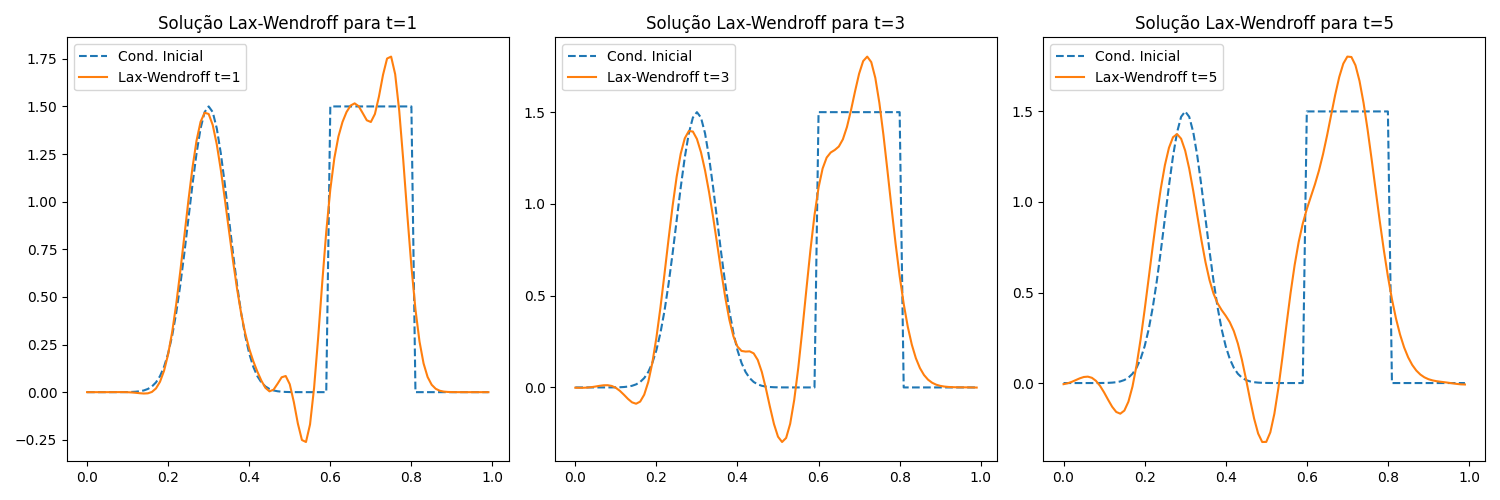
\includegraphics[width=\textwidth]{code/images/Lax-Wendroff.png}
    \caption{Solução Lax-Wendroff para $t=1$, $t=3$, e $t=5$, com a condição inicial representada pela linha tracejada.}
\end{figure}

\begin{table}[H]
    \centering
    \begin{tabular}{lrrrrr}
\toprule
 & Posição Espacial & Cond. Inicial & Lax-Wendroff t=1 & Lax-Wendroff t=3 & Lax-Wendroff t=5 \\
\midrule
0 & 0.000000 & 0.000000 & 0.000080 & 0.011905 & 0.055474 \\
1 & 0.050000 & 0.000006 & 0.001377 & 0.023119 & 0.065938 \\
2 & 0.100000 & 0.000503 & 0.014635 & 0.079522 & 0.137594 \\
3 & 0.150000 & 0.016663 & 0.094425 & 0.215688 & 0.270011 \\
4 & 0.200000 & 0.203003 & 0.365367 & 0.445116 & 0.443586 \\
5 & 0.250000 & 0.909796 & 0.836718 & 0.694310 & 0.602054 \\
6 & 0.300000 & 1.500000 & 1.117720 & 0.813352 & 0.673555 \\
7 & 0.350000 & 0.909796 & 0.857233 & 0.711728 & 0.624466 \\
8 & 0.400000 & 0.203003 & 0.371055 & 0.469340 & 0.496815 \\
9 & 0.450000 & 0.016663 & 0.090523 & 0.266608 & 0.388061 \\
10 & 0.500000 & 0.000503 & 0.041207 & 0.241638 & 0.389089 \\
11 & 0.550000 & 0.000006 & 0.236351 & 0.434262 & 0.529188 \\
12 & 0.600000 & 1.500000 & 0.803478 & 0.776761 & 0.758244 \\
13 & 0.650000 & 1.500000 & 1.338980 & 1.102181 & 0.970629 \\
14 & 0.700000 & 1.500000 & 1.472451 & 1.237641 & 1.060403 \\
15 & 0.750000 & 1.500000 & 1.333151 & 1.114042 & 0.978795 \\
16 & 0.800000 & 1.500000 & 0.829878 & 0.791623 & 0.758141 \\
17 & 0.850000 & 0.000000 & 0.235362 & 0.424940 & 0.487426 \\
18 & 0.900000 & 0.000000 & 0.019660 & 0.163072 & 0.257071 \\
19 & 0.950000 & 0.000000 & 0.000293 & 0.043092 & 0.113403 \\
\bottomrule
\end{tabular}

    \caption{Tabela de resultados para o método Lax-Wendroff nas posições espaciais selecionadas e diferentes tempos}
    \label{tab:lax_wendroff}
\end{table}

\subsection{Análise dos Resultados do Método Lax-Wendroff}

O método Lax-Wendroff, sendo de segunda ordem, oferece uma precisão maior que o método Upwind ao reduzir a dissipação numérica, mas pode introduzir oscilações indesejadas em torno de descontinuidades. Na Figura , observamos que para \( t=1 \), a solução mantém bem o perfil da condição inicial. No entanto, para \( t=3 \) e \( t=5 \), começam a surgir pequenas oscilações nas regiões de transição, típicas deste método. Essas oscilações são resultado da aproximação de alta ordem e podem ser amenizadas com métodos adicionais de controle de oscilação.

\subsection{Implementação em Python}

O código em Python é utilizado para resolver a advecção com o método Lax-Wendroff, aplicando condições de contorno periódicas. O código é estruturado com uma função principal \texttt{resolverAdveccao} para calcular a solução da advecção para diferentes métodos numéricos e uma função específica para o método Lax-Wendroff.

\begin{lstlisting}[language=Python, caption={Código para resolver a advecção usando o método Lax-Wendroff}, label={lst:codigo_lax_wendroff}]
# Função para resolver a advecção com diferentes métodos numéricos
def resolverAdveccao(metodo, condicaoInicial, intervaloTempo, intervaloEspacial, numeroCourant, tempoFinal):
    """
    Calcula a solução da advecção para um determinado método e tempo final.
    """
    densidade = condicaoInicial.copy()
    tempoAtual = 0
    while tempoAtual < tempoFinal:
        densidade = metodo(densidade, intervaloTempo, intervaloEspacial, numeroCourant)
        tempoAtual += intervaloTempo
    return densidade

# Método Lax-Wendroff com condições de contorno periódicas
def metodoLaxWendroff(densidade, intervaloTempo, intervaloEspacial, numeroCourant):
    """
    Calcula a solução de advecção usando o método Lax-Wendroff.
    """
    novaDensidade = densidade.copy()
    for i in range(numPontosEspaco):
        novaDensidade[i] = densidade[i] - 0.5 * numeroCourant * (densidade[(i+1) \% numPontosEspaco] - densidade[i-1]) + \
                            0.5 * numeroCourant**2 * (densidade[i-1] - 2 * densidade[i] + densidade[(i+1) \% numPontosEspaco])
    return novaDensidade

# Cálculo da densidade para diferentes tempos
densidadeLaxWendroff1 = resolverAdveccao(metodoLaxWendroff, condicaoInicial, intervaloTempo, intervaloEspacial, numeroCourant, tempoFinal1)
densidadeLaxWendroff3 = resolverAdveccao(metodoLaxWendroff, condicaoInicial, intervaloTempo, intervaloEspacial, numeroCourant, tempoFinal3)
densidadeLaxWendroff5 = resolverAdveccao(metodoLaxWendroff, condicaoInicial, intervaloTempo, intervaloEspacial, numeroCourant, tempoFinal5)
\end{lstlisting}

A função \texttt{resolverAdveccao} calcula a evolução da densidade ao longo do tempo até atingir o tempo final especificado. A função \texttt{metodoLaxWendroff} implementa o método Lax-Wendroff para calcular a nova densidade em cada ponto do espaço, utilizando o número de Courant especificado.
